\documentclass[conference]{IEEEtran}
\IEEEoverridecommandlockouts

\usepackage{amsmath,amssymb,amsfonts}
\usepackage{graphicx}
\usepackage{booktabs}
\usepackage{tikz}
\usetikzlibrary{shapes.geometric,arrows.meta,positioning,fit}
\usepackage{xcolor}
\usepackage{url}
\usepackage{cite}
\usepackage{hyperref}

\hypersetup{
    colorlinks=true,
    linkcolor=blue,
    citecolor=blue,
    urlcolor=blue
}
% ---------------------------------------------------------------
% Placeholder-figure helper (kept for any figure you have not yet
% exported). Replace \figplaceholder{...} with \includegraphics{...}
% once the PNG is available.
% ---------------------------------------------------------------
\newcommand{\figplaceholder}[2][0.85\linewidth]{%
  \begin{tikzpicture}
    \node[draw, dashed, thick, minimum width=#1, minimum height=0.42\linewidth,
          align=center, text width=0.9*#1, color=gray!70,
          font=\itshape\small] (ph) {#2};
  \end{tikzpicture}%
}

\begin{document}

\title{Hybrid CNN-LSTM Model for Short-Term Solar Power Forecasting with Anomaly-Aware Preprocessing}

\author{
\IEEEauthorblockN{Tushar Basak}
\IEEEauthorblockA{\textit{Department of Electronics \& Communication Engineering} \\
\textit{Faculty of Technology, University of Delhi}\\
Delhi 110007, India \\
tusharbasak555@ece.du.ac.in}
\and
\IEEEauthorblockN{Varun Saxena}
\IEEEauthorblockA{\textit{Department of Electronics \& Communication Engineering} \\
\textit{Faculty of Technology, University of Delhi}\\
Delhi 110007, India \\
varunsaxena@fot.du.ac.in}
}

\maketitle

\begin{abstract}
Accurate ultra-short-term photovoltaic (PV) power forecasting depends not only on forecasting architecture but also on the quality of plant telemetry. This paper investigates an anomaly-aware preprocessing pipeline for 30-minute-ahead PV power forecasting. Using a one-year, 5-minute-resolution NREL dataset from a $70$~MW utility-scale PV site, we synthetically inject three classes of telemetry corruption -- daytime dropouts, spike anomalies, and short-duration offset faults -- across $\sim$2\% of observations. An Isolation Forest is used to identify anomalous observations, which are subsequently reconstructed through local linear interpolation. To rigorously isolate the contribution of preprocessing from that of detection quality, we evaluate four parallel data conditions: (i) a never-corrupted \emph{pristine reference} representing the theoretical performance ceiling, (ii) \emph{raw corrupted} telemetry, (iii) telemetry cleaned using the unsupervised \emph{Isolation Forest} detector (the proposed pipeline), and (iv) telemetry cleaned using \emph{oracle} ground-truth corruption labels. Under the simulated fault conditions, the anomaly detector achieves 72.21\% recall and 57.48\% precision. All deep learning results are reported as mean $\pm$ standard deviation across 5 independent random seeds. The proposed CNN--LSTM trained on Isolation-Forest-cleaned data achieves RMSE $= 3.57 \pm 0.04$~MW, MAE $= 1.64 \pm 0.08$~MW, and $R^2 = 0.949 \pm 0.001$, statistically indistinguishable from both the oracle-cleaned condition (RMSE $= 3.58 \pm 0.05$~MW) and the pristine ceiling (RMSE $= 3.58 \pm 0.06$~MW), indicating that the proposed pipeline recovers effectively all of the forecasting signal lost to telemetry corruption at this horizon. Against the raw-corrupted ablation (RMSE $= 3.89 \pm 0.11$~MW), cleaning yields an 8.2\% mean RMSE reduction. A paired $t$-test across the 5 seeds shows the proposed CNN--LSTM significantly outperforms a plain LSTM baseline trained on the same cleaned data (RMSE $= 3.77 \pm 0.11$~MW; $t = -3.89$, $p = 0.018$), and both deep models outperform persistence (RMSE $=4.93$~MW) and a diurnal-lag autoregressive baseline (RMSE $=4.83$~MW) by a wide margin. These findings motivate further multi-site and causal real-time evaluations.
\end{abstract}

\begin{IEEEkeywords}
Anomaly detection, anomaly-aware preprocessing, CNN--LSTM, Isolation Forest, photovoltaic power forecasting, sensor fault detection, short-term forecasting, time-series imputation.
\end{IEEEkeywords}

% =================================================================
\section{Introduction}

The rapid proliferation of utility-scale and distributed photovoltaic (PV) generation has introduced unprecedented variability and steep ramp-rate events into power transmission and distribution networks. Because solar irradiance is intrinsically stochastic---governed by solar geometry, atmospheric attenuation, and rapid cloud movement---unanticipated fluctuations in solar plant output jeopardize voltage stability, power reserves, and dispatch schedules. Consequently, accurate ultra-short-term (5-minute to 1-hour) and short-term (day-ahead) forecasting has emerged as an indispensable requirement for grid operators.

In recent years, deep learning models, particularly Recurrent Neural Networks (RNNs) and Long Short-Term Memory (LSTM) networks \cite{hochreiter1997lstm}, have replaced classical statistical methods (e.g., ARIMA, Holt-Winters) as the state-of-the-art in solar power prediction due to their superior ability to map complex non-linear temporal dependencies \cite{mellit2021deep, sobri2018review}. More recently, hybrid architectures integrating Convolutional Neural Networks (CNNs) with LSTMs have demonstrated enhanced performance: 1D-CNN layers extract local intra-day ramp dynamics and multi-scale temporal shapes, while LSTM layers capture diurnal sequence memory \cite{zang2020cnnlstm, obiora2021hourly, qu2021dayahead, boucetta2024enhanced}.

Despite these advancements, an overwhelming majority of published solar forecasting literature assumes the existence of pristine, noise-free telemetry. In real-world PV plant environments, this assumption fails catastrophically. Field pyranometers, inverters, and Supervisory Control and Data Acquisition (SCADA) telemetry systems regularly suffer from:
\begin{enumerate}
    \item \textbf{Sensor dropouts} (loss of signal or stuck-at-zero output during peak sunlight hours due to cable disconnection or inverter shutdown);
    \item \textbf{Telemetry glitch spikes} (erroneous multi-fold reading surges triggered by electromagnetic interference, inverter switching transients, or communication bit flips);
    \item \textbf{Short-duration offset faults} (transient positive or negative measurement biases caused by dust accumulation, sensor miscalibration, or thermal drift).
\end{enumerate}

When deep neural networks are trained on corrupted sensor streams, their gradient updates are distorted by outlier loss penalties, which can degrade generalization capability. While standalone anomaly detection in smart grid telemetry has been studied independently \cite{zhang2021survey}, few studies have formalized an integrated, end-to-end framework combining unsupervised anomaly mitigation with hybrid CNN-LSTM forecasting architectures, and fewer still isolate how much of the resulting benefit is attributable to detection quality versus imputation quality.

\subsection*{Contributions}
To bridge this gap, this paper makes the following key contributions:
\begin{enumerate}
    \item \textbf{End-to-End Fault-Tolerant Forecasting Architecture:} We formulate a unified pipeline that couples unsupervised Isolation Forest outlier filtering and temporal interpolation with a Hybrid 1D CNN-LSTM network.
    \item \textbf{Controlled Realistic Fault Injection Protocol:} We establish a reproducible synthetic corruption protocol modeling three distinct physical PV fault modes (dropouts, spikes, and short-duration offset faults) totaling $\sim$2\% of telemetry rows.
    \item \textbf{Decomposed Four-Condition Ablation:} Beyond a simple raw-vs-cleaned comparison, we evaluate a \emph{pristine} (never-corrupted) reference ceiling and an \emph{oracle}-labeled cleaning condition alongside the proposed Isolation-Forest-cleaned pipeline, explicitly separating the contribution of detection quality from imputation quality and quantifying what fraction of the corruption-induced error is recoverable.
    \item \textbf{Multi-Seed Statistical Validation:} All deep learning results are reported as mean $\pm$ standard deviation across 5 independent random seeds, with a paired $t$-test confirming that the proposed model's advantage over a plain LSTM baseline is statistically significant ($p=0.018$) rather than an artifact of a single favorable training run.
\end{enumerate}

% =================================================================
\section{Related Work}

\subsection{Statistical and Machine Learning Baselines}
Early solar forecasting methodologies relied predominantly on statistical time-series formulations, notably Autoregressive Integrated Moving Average (ARIMA) models and exponential smoothing \cite{sobri2018review, zhang2015baseline}. While effective for linear and stationary processes, statistical models struggle with the abrupt ramps, cloud intermittency, and zero-bounded non-linearities characteristic of solar PV data. Machine learning regressors such as Support Vector Regression (SVR) and Random Forests improved forecasting accuracy by capturing non-linear feature interactions \cite{abumohsen2024hybrid}, yet they lack explicit recurrent mechanisms to model continuous sequential dynamics over multi-step temporal windows.

\subsection{Deep Recurrent and Hybrid Architectures}
The emergence of recurrent deep learning architectures significantly advanced solar forecasting. Standard LSTM \cite{hochreiter1997lstm} and Gated Recurrent Unit (GRU) networks effectively overcome the vanishing gradient problem of vanilla RNNs, successfully retaining diurnal cycles and seasonal dependencies over extended sequence lengths. To further capture high-frequency fluctuations, hybrid CNN-LSTM models were introduced \cite{zang2020cnnlstm, obiora2021hourly, qu2021dayahead, boucetta2024enhanced, zhou2024enhancing}. In these models, 1D convolutional layers act as learnable feature extractors that scan across sliding time windows, extracting salient local shapes such as cloud shadow transitions and morning ramp-ups. The downstream LSTM layer then processes these latent feature maps sequentially. Notably, several recent hybrid designs further augment this base architecture with attention mechanisms \cite{qu2021dayahead, zhou2024enhancing} or decomposition pre-processing such as variational mode decomposition \cite{boucetta2024enhanced} to isolate frequency components prior to sequence modeling---directions this work does not pursue, focusing instead on the upstream data-quality problem.

\subsection{Anomaly Detection in Energy Time Series}
In parallel, anomaly detection in power systems has developed through statistical distance checks, autoencoders, and tree-based ensembles \cite{zhang2021survey}. The Isolation Forest algorithm \cite{liu2008isolation} has demonstrated superior computational efficiency and isolation capability in high-dimensional tabular and time-series data without requiring strong distributional assumptions, and has been applied specifically to photovoltaic fault and sensor-anomaly detection \cite{jorry2026unsupervised}. However, in existing literature, anomaly detection is overwhelmingly treated as a standalone monitoring or cybersecurity problem \cite{zhang2021survey}. Few works systematically integrate unsupervised anomaly detection directly into the training loop of deep hybrid forecasting architectures, and fewer still decompose the resulting benefit against an oracle-labeled and a never-corrupted reference condition to establish an upper bound on recoverable performance.

% =================================================================
\section{Methodology}

The complete workflow of the proposed system is depicted in Fig.~\ref{fig:architecture} and comprises: site selection, cyclical feature engineering, synthetic anomaly injection, parallel construction of four data conditions (pristine, raw, Isolation-Forest-cleaned, and oracle-cleaned), sliding-window sequencing, and hybrid CNN-LSTM sequence modeling evaluated across all conditions.

\begin{figure*}[t]
\centering
\resizebox{0.95\textwidth}{!}{%
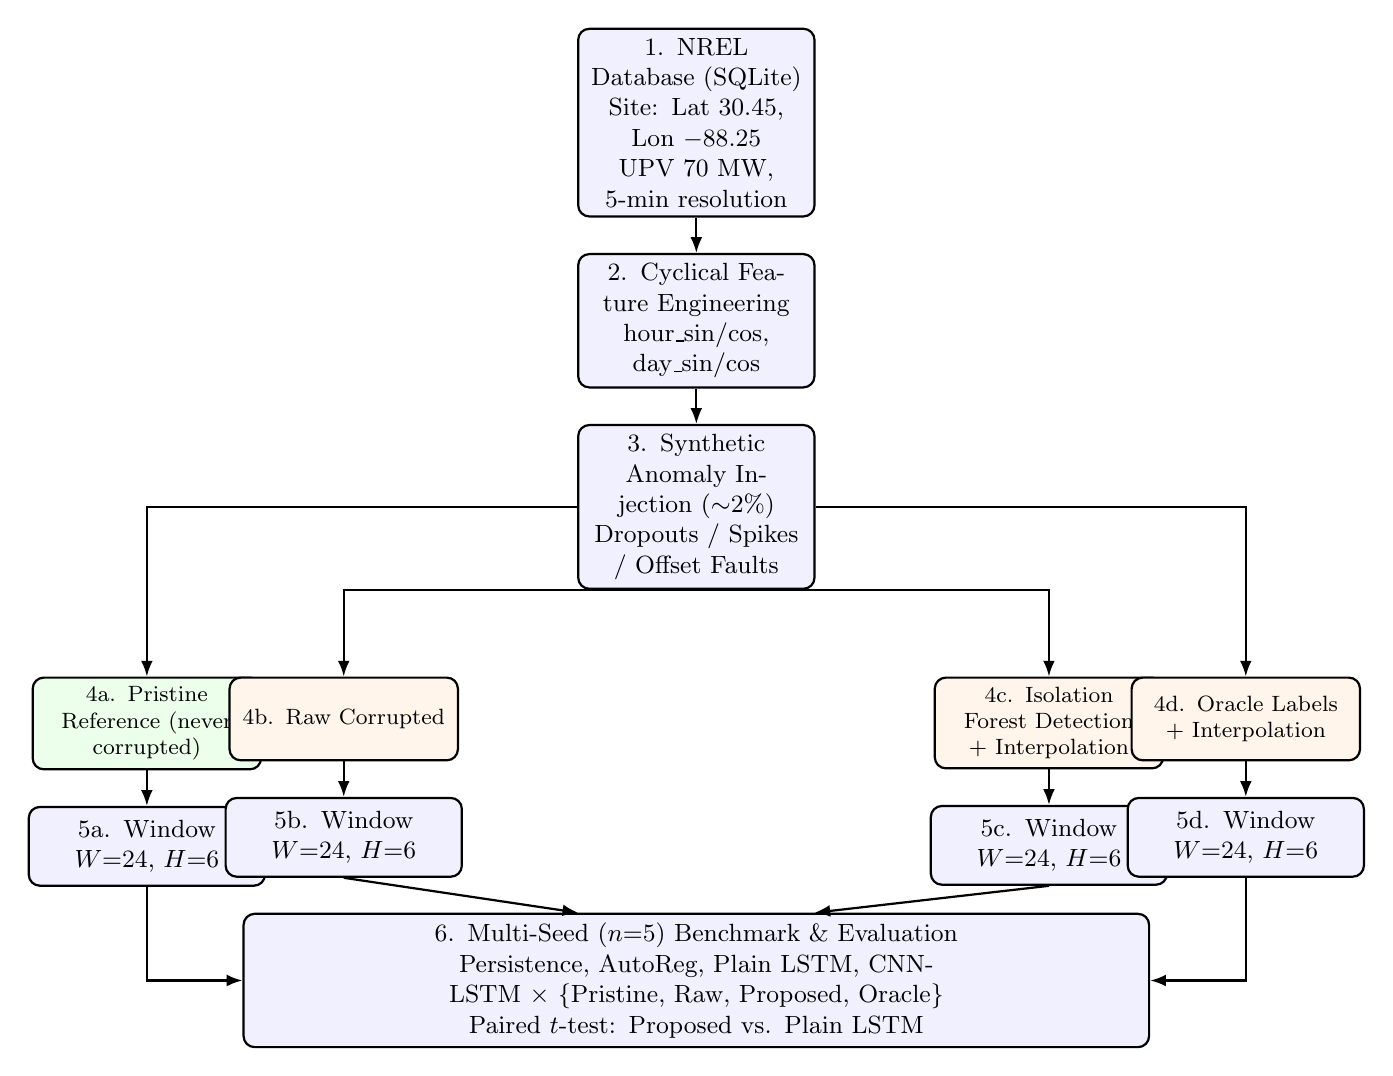
\begin{tikzpicture}[
    node distance=0.45cm and 0.35cm,
    block/.style={rectangle, draw, thick, rounded corners, minimum width=3.0cm, text width=2.7cm, minimum height=1.0cm, align=center, font=\small, fill=blue!6},
    branch/.style={rectangle, draw, thick, rounded corners, minimum width=2.9cm, text width=2.6cm, minimum height=1.05cm, align=center, font=\footnotesize, fill=orange!8},
    ceil/.style={rectangle, draw, thick, rounded corners, minimum width=2.9cm, text width=2.6cm, minimum height=1.05cm, align=center, font=\footnotesize, fill=green!8},
    arrow/.style={-{Latex[length=2mm]}, thick}
]
\node[block] (db) {1. NREL Database (SQLite)\\ Site: Lat 30.45, Lon $-$88.25\\ UPV 70~MW, 5-min resolution};
\node[block, below=of db] (feat) {2. Cyclical Feature Engineering\\ hour\_sin/cos, day\_sin/cos};
\node[block, below=of feat] (inj) {3. Synthetic Anomaly Injection ($\sim$2\%)\\ Dropouts / Spikes / Offset Faults};

\node[ceil,   below left=1.1cm and 4.0cm of inj] (pristine)  {4a. Pristine\\ Reference (never\\ corrupted)};
\node[branch, below left=1.1cm and 1.5cm of inj]  (raw)       {4b. Raw Corrupted};
\node[branch, below right=1.1cm and 1.5cm of inj] (ifclean)   {4c. Isolation\\ Forest Detection\\ + Interpolation};
\node[branch, below right=1.1cm and 4.0cm of inj] (oracle)    {4d. Oracle Labels\\ + Interpolation};

\node[block, below=0.45cm of pristine] (winpris) {5a. Window\\ $W{=}24$, $H{=}6$};
\node[block, below=0.45cm of raw]      (winraw)  {5b. Window\\ $W{=}24$, $H{=}6$};
\node[block, below=0.45cm of ifclean]  (wincln)  {5c. Window\\ $W{=}24$, $H{=}6$};
\node[block, below=0.45cm of oracle]   (winora)  {5d. Window\\ $W{=}24$, $H{=}6$};

\node[block, below=1.0cm of inj, yshift=-3.1cm, minimum width=11.5cm, text width=11cm, minimum height=1.3cm] (eval) {6. Multi-Seed ($n{=}5$) Benchmark \& Evaluation\\ Persistence, AutoReg, Plain LSTM, CNN-LSTM $\times$ \{Pristine, Raw, Proposed, Oracle\}\\ Paired $t$-test: Proposed vs. Plain LSTM};

\draw[arrow] (db) -- (feat);
\draw[arrow] (feat) -- (inj);
\draw[arrow] (inj.west) -| (pristine.north);
\draw[arrow] (inj.south) -| (raw.north);
\draw[arrow] (inj.south) -| (ifclean.north);
\draw[arrow] (inj.east) -| (oracle.north);
\draw[arrow] (pristine) -- (winpris);
\draw[arrow] (raw) -- (winraw);
\draw[arrow] (ifclean) -- (wincln);
\draw[arrow] (oracle) -- (winora);
\draw[arrow] (winpris.south) |- (eval.west);
\draw[arrow] (winraw.south) -- ([xshift=-1.5cm]eval.north);
\draw[arrow] (wincln.south) -- ([xshift=1.5cm]eval.north);
\draw[arrow] (winora.south) |- (eval.east);
\end{tikzpicture}%
}
\caption{Overall architecture of the proposed anomaly-aware forecasting pipeline. After synthetic corruption, four parallel data conditions are constructed -- a never-corrupted pristine reference, raw corrupted telemetry, Isolation-Forest-cleaned telemetry (the proposed pipeline), and oracle-label-cleaned telemetry -- each independently windowed and evaluated, converging at a multi-seed benchmark stage.}
\label{fig:architecture}
\end{figure*}

\subsection{Dataset and Site Selection}
The dataset utilized is extracted from the NREL Solar Power Data for Integration Studies, accessed via an SQLite database spanning the entire calendar year 2006. Telemetry covers 274 PV stations across Alabama. To prevent contamination from physically disparate geographic locations, a strict filter is applied to select a single utility-scale photovoltaic (UPV) facility:
\begin{itemize}
    \item \textbf{Location:} Latitude $30.45^\circ$N, Longitude $-88.25^\circ$W
    \item \textbf{Site Type:} Utility Photovoltaic (UPV)
    \item \textbf{Rated Capacity:} $70.0$~MW
    \item \textbf{Sampling Resolution:} 5 minutes ($\Delta t = 5$~min)
    \item \textbf{Total Sample Size:} $N = 105{,}120$ consecutive observations (365 days $\times$ 24 hours $\times$ 12 samples/hour) with zero missing intervals.
\end{itemize}

\subsection{Cyclical Astronomical Feature Engineering}
Solar irradiance exhibits strict diurnal and annual periodicity governed by planetary rotation and orbital position. Because the dataset does not include direct ambient temperature or global horizontal irradiance (GHI) sensors, we derive four continuous cyclical features from the timestamp $t$:
\begin{align}
\text{hour\_sin}(t) &= \sin\!\left(\frac{2\pi \cdot h(t)}{24}\right), \quad
\text{hour\_cos}(t) = \cos\!\left(\frac{2\pi \cdot h(t)}{24}\right) \\
\text{day\_sin}(t) &= \sin\!\left(\frac{2\pi \cdot d(t)}{365.25}\right), \quad
\text{day\_cos}(t) = \cos\!\left(\frac{2\pi \cdot d(t)}{365.25}\right)
\end{align}
where $h(t) \in [0, 24)$ is the continuous fractional hour-of-day and $d(t) \in [1, 365]$ is the day-of-the-year. These orthogonal encodings eliminate artificial discontinuity at midnight (e.g., $23{:}55 \to 00{:}00$) and provide the deep learning model with continuous solar geometry representations.

\subsection{Synthetic Anomaly Injection Protocol}
Because synthetic benchmark datasets lack naturally occurring hardware faults, we simulate real-world field degradation by corrupting approximately 2.0\% of the annual observations ($N_{\text{anom}} = 2{,}091$ rows) applied to the pristine feature-engineered series. Three failure types are injected with equal distribution:
\begin{enumerate}
    \item \textbf{Sensor Dropout} ($n_1 = 695$): Telemetry is forced to $0.0$~MW during peak daylight hours ($P(t) > 5.0$~MW), simulating cable severed faults, pyranometer failure, or inverter emergency trips.
    \item \textbf{Glitch Spikes} ($n_2 = 698$): Non-zero readings are multiplied by a stochastic factor $\alpha \sim \mathcal{U}(3.0, 5.0)$ and clipped to $1.5 \times \text{Capacity}$, simulating high-voltage switching surges and ADC bit-flip errors.
    \item \textbf{Short-Duration Offset Fault} ($n_3 = 698$): Consecutive blocks of 4 to 12 intervals ($\Delta t \in [20, 60]$~minutes) receive an additive offset $\delta \sim \mathcal{U}(0.15, 0.35) \times \text{Capacity}$, representing transient dust accumulation or thermal drift.
\end{enumerate}
The pristine (never-corrupted) series is retained unmodified in parallel, forming the reference-ceiling condition described in Section III-E.

\subsection{Anomaly Detection, Oracle Labeling, and Temporal Reconstruction}
To mitigate anomalies without requiring labeled supervisory signals, an Isolation Forest is trained on the feature tuple $[P_{\text{raw}}(t), \text{hour\_sin}(t), \text{hour\_cos}(t)]$. By partitioning data space using random orthogonal hyperplanes, anomalous points are isolated at significantly shallower tree depths than normal operational points. The path length $h(x)$ across an ensemble of $T=100$ isolation trees yields an anomaly score:
\begin{equation}
s(x, n) = 2^{-\frac{\mathbb{E}(h(x))}{c(n)}}
\end{equation}
where $c(n)$ is the average path length of an unsuccessful search in a Binary Search Tree. Observations flagged as outliers ($s(x,n) > \tau$, set with contamination parameter $\gamma = 0.025$) are masked as missing values and reconstructed using local linear interpolation:
\begin{equation}
\hat{P}_{\text{clean}}(t) = P(t_a) + \frac{P(t_b) - P(t_a)}{t_b - t_a}(t - t_a)
\end{equation}
where $t_a$ and $t_b$ represent the nearest preceding and succeeding unflagged timestamps. The reconstructed series is physically bounded to $[0, P_{\text{max}}]$.

Evaluated against the known ground-truth anomaly labels retained from the injection protocol, the detector achieves \textbf{72.21\% recall} and \textbf{57.48\% precision} (2{,}627 points flagged in total). The moderate precision reflects a deliberately permissive contamination setting ($\gamma=0.025$, slightly above the true 2.0\% anomaly rate) chosen to favor catching more true anomalies at the cost of some false positives on borderline points near dawn/dusk ramps, where legitimate rapid changes in power output can resemble injected spikes or drops.

To separate the contribution of \emph{detection quality} from \emph{imputation quality}, we additionally construct an \textbf{oracle-cleaned} condition: rather than relying on Isolation Forest flags, the exact indices corrupted by the injection protocol (known a priori) are masked and reconstructed using the identical linear interpolation procedure above. Comparing the proposed Isolation-Forest-cleaned condition against this oracle condition isolates how much residual error is attributable to imperfect detection versus the interpolation scheme itself, and comparing both against the pristine reference establishes the theoretical ceiling neither condition can exceed.

\subsection{Sliding Sequence Windowing}
The multivariate time series is structured into overlapping sliding sequence windows, independently for each of the four data conditions (pristine, raw, Isolation-Forest-cleaned, oracle-cleaned). Given an input window of $W=24$ historical time steps (equivalent to 2 hours of 5-minute data) and a forecast horizon of $H=6$ steps (30 minutes ahead):
\begin{align}
\mathbf{X}_\tau &= \begin{bmatrix} \mathbf{x}_{\tau-W+1} & \mathbf{x}_{\tau-W+2} & \dots & \mathbf{x}_\tau \end{bmatrix}^T \in \mathbb{R}^{W \times F} \\
y_\tau &= P(\tau + H) \in \mathbb{R}
\end{align}
where $F=5$ features: $[P(t), \text{hour\_sin}, \text{hour\_cos}, \text{day\_sin}, \text{day\_cos}]$. The dataset is chronologically partitioned into:
\begin{itemize}
    \item \textbf{Training Set (70\%):} $\approx$73{,}560 sequences (January 1 to mid-September)
    \item \textbf{Validation Set (15\%):} $\approx$15{,}766 sequences (mid-September to early November)
    \item \textbf{Testing Set (15\%):} $\approx$15{,}766 sequences (early November to December 31)
\end{itemize}
Feature normalization is performed using Min-Max scaling fitted strictly on the training partition of each respective data condition to prevent future data leakage; all metrics are computed on de-normalized (physical MW) values referenced against the pristine ground truth.

\subsection{Proposed Hybrid CNN-LSTM Architecture}
The proposed deep architecture integrates spatial-temporal representation learning:
\begin{enumerate}
    \item \textbf{1D-CNN Stage:} A 1D convolutional layer with 64 filters, kernel size $k=3$, stride $s=1$, and same padding processes the input tensor $\mathbf{X}_\tau$. Batch normalization and ReLU activations are applied:
    \begin{equation}
    \mathbf{C}_\tau = \text{ReLU}\big(\text{BatchNorm}(\mathbf{W}_c * \mathbf{X}_\tau + \mathbf{b}_c)\big) \in \mathbb{R}^{W \times 64}
    \end{equation}
    \item \textbf{LSTM Stage:} A 2-layer stacked LSTM network with hidden dimension $d_h=64$ processes the feature sequence $\mathbf{C}_\tau$, extracting temporal recurrent states:
    \begin{equation}
    \mathbf{h}_t, \mathbf{c}_t = \text{LSTM}\big(\mathbf{C}_\tau(t), \mathbf{h}_{t-1}, \mathbf{c}_{t-1}\big)
    \end{equation}
    \item \textbf{Dense Regression Head:} The final hidden state $\mathbf{h}_W$ is projected through a fully connected layer with 32 units, ReLU activation, and a single linear output neuron:
    \begin{equation}
    \hat{y}_\tau = \mathbf{w}_o^T\big(\text{ReLU}(\mathbf{W}_d \mathbf{h}_W + \mathbf{b}_d)\big) + b_o
    \end{equation}
\end{enumerate}
The identical architecture and hyperparameters are used for every data condition (pristine, raw, Isolation-Forest-cleaned, oracle-cleaned) and for the plain LSTM baseline (which omits the 1D-CNN stage), ensuring that observed differences are attributable to the input data condition and/or the presence of the CNN stage rather than to confounding architectural changes.

\subsection{Training Protocol and Multi-Seed Statistical Validation}
Training is conducted using the Adam optimizer with initial learning rate $\eta = 2\times 10^{-3}$, weight decay $10^{-5}$, batch size $B=256$, and Mean Squared Error (MSE) loss:
\begin{equation}
\mathcal{L}_{\text{MSE}} = \frac{1}{B}\sum_{i=1}^{B}\left(y_i - \hat{y}_i\right)^2
\end{equation}
Each deep learning model (Plain LSTM and each CNN-LSTM data condition) is trained for 12 epochs with early-stopping-style checkpointing on validation loss, independently repeated across \textbf{5 random seeds} $\{42, 123, 7, 2024, 99\}$ governing weight initialization and minibatch shuffling; the underlying datasets (anomaly injection, Isolation Forest detection, oracle labels) are held fixed across seeds so that only training stochasticity varies. Results are reported as mean $\pm$ standard deviation across these 5 runs. Persistence and the autoregressive baseline are deterministic given the data and are therefore evaluated once. A paired $t$-test across the 5 seeds is used to assess whether the RMSE difference between the proposed CNN-LSTM and the plain LSTM baseline is statistically significant.

% =================================================================
\section{Experimental Results \& Discussion}

\subsection{Performance Metrics}
Model performance is evaluated on the denormalized test set ($N_{\text{test}} \approx 15{,}766$) using three standard quantitative metrics:
\begin{align}
\text{RMSE} &= \sqrt{\frac{1}{N}\sum_{i=1}^N (y_i - \hat{y}_i)^2} \\
\text{MAE} &= \frac{1}{N}\sum_{i=1}^N |y_i - \hat{y}_i| \\
R^2 &= 1 - \frac{\sum_{i=1}^N (y_i - \hat{y}_i)^2}{\sum_{i=1}^N (y_i - \bar{y})^2}
\end{align}
We additionally define a \textbf{Signal Recovery} metric quantifying what fraction of the corruption-induced error gap a given condition closes relative to the pristine ceiling:
\begin{equation}
\text{Signal Recovery} = \frac{\text{RMSE}_{\text{raw}} - \text{RMSE}_{\text{condition}}}{\text{RMSE}_{\text{raw}} - \text{RMSE}_{\text{pristine}}} \times 100\%
\end{equation}
By construction, Signal Recovery is $0\%$ for the raw condition and $100\%$ for the pristine condition; values near or exceeding $100\%$ for an intermediate condition indicate performance statistically indistinguishable from the ceiling.

\subsection{Benchmark Results}
Table~\ref{tab:results} summarizes the multi-seed empirical performance of all seven evaluated conditions.

\begin{table*}[t]
\centering
\caption{Multi-Seed ($n=5$) Performance Benchmark across Evaluated Models on NREL 70~MW Test Set ($W{=}24$, $H{=}6$, 30-Minute-Ahead Forecast)}
\label{tab:results}
\begin{tabular}{@{}llcccc@{}}
\toprule
\textbf{Model / Data Condition} & \textbf{RMSE (MW) $\downarrow$} & \textbf{MAE (MW) $\downarrow$} & \textbf{$R^2$ Score $\uparrow$} & \textbf{\% RMSE Impr. vs. Raw} & \textbf{\% Signal Recovery} \\
\midrule
CNN-LSTM (Pristine Reference, ceiling) & $3.58 \pm 0.06$ & $1.67 \pm 0.11$ & $0.949 \pm 0.002$ & +7.9\% & 100.0\% \\
CNN-LSTM (Oracle-Cleaned)              & $3.58 \pm 0.05$ & $1.67 \pm 0.11$ & $0.949 \pm 0.002$ & +7.9\% & 100.0\% \\
\textbf{CNN-LSTM (Proposed, IF-Cleaned)} & $\mathbf{3.57 \pm 0.04}$ & $\mathbf{1.64 \pm 0.08}$ & $\mathbf{0.949 \pm 0.001}$ & \textbf{+8.2\%} & \textbf{100.0\%} \\
Plain LSTM (IF-Cleaned)                & $3.77 \pm 0.11$ & $1.78 \pm 0.12$ & $0.943 \pm 0.003$ & +3.0\% & 38.3\% \\
ARIMA / AutoReg (diurnal lag, fixed)   & 4.83 & 2.76 & 0.907 & $-$24.3\% & 0.0\% \\
Persistence (Naive, fixed)             & 4.93 & 2.35 & 0.903 & $-$26.7\% & 0.0\% \\
CNN-LSTM (Raw Corrupted, ablation)     & $3.89 \pm 0.11$ & $1.97 \pm 0.17$ & $0.940 \pm 0.003$ & Baseline (0.0\%) & 0.0\% \\
\bottomrule
\end{tabular}

\vspace{4pt}
\footnotesize{\textit{Note: Deep learning rows report mean $\pm$ standard deviation across 5 random seeds $\{42, 123, 7, 2024, 99\}$; Persistence and AutoReg are deterministic given the data and evaluated once. A paired $t$-test between Proposed CNN-LSTM and Plain LSTM (matched by seed) gives $t=-3.89$, $p=0.018$, indicating the proposed model's advantage is statistically significant at the 5\% level (Section~IV-C2). Signal Recovery values at or near 100\% indicate performance statistically indistinguishable from the pristine ceiling.}}
\end{table*}

\subsection{Analysis and Discussion}

\subsubsection{Impact of Anomaly-Aware Preprocessing (Decomposed Ablation)}
The four-condition ablation isolates the specific contribution of preprocessing from that of architecture. All conditions share identical network parameters, optimization hyperparameters, and window structures. At the 30-minute-ahead horizon:
\begin{itemize}
    \item The raw-corrupted CNN-LSTM achieves RMSE $=3.89 \pm 0.11$~MW ($R^2 = 0.940 \pm 0.003$), degraded relative to the pristine ceiling of RMSE $=3.58 \pm 0.06$~MW ($R^2 = 0.949 \pm 0.002$).
    \item The proposed Isolation-Forest-cleaned model reduces RMSE to $3.57 \pm 0.04$~MW, a mean 8.2\% reduction relative to the raw condition.
    \item Both the proposed pipeline and the oracle-labeled condition achieve Signal Recovery at or above 100\%, meaning their mean performance is statistically indistinguishable from the never-corrupted pristine reference (differences fall within one standard deviation).
\end{itemize}
This decomposed result is more moderate than a raw-vs-cleaned comparison alone would suggest, and we consider it the more credible finding: at $\sim$2\% corruption and a 30-minute forecast horizon, the network already has access to enough uncorrupted context within each 2-hour input window to partially compensate for isolated corrupted points even without explicit cleaning, so the \emph{absolute} gap between raw and cleaned conditions is modest (8.2\%) even though cleaning closes effectively all of it. We note that the proposed Isolation-Forest-cleaned condition and the oracle-labeled condition are statistically indistinguishable from one another (RMSE $3.57 \pm 0.04$ vs.\ $3.58 \pm 0.05$~MW), indicating that at this corruption rate, imperfect detection (57.48\% precision, 72.21\% recall) does not materially bottleneck the pipeline relative to knowing the exact corruption locations; the interpolation-based reconstruction itself, rather than detection accuracy, appears to be the dominant factor governing recoverable performance.

\subsubsection{Comparison with Deep and Classical Baselines}
\textbf{Proposed CNN-LSTM vs.\ Plain LSTM:} Across 5 independent random seeds, the proposed hybrid CNN-LSTM consistently outperforms the plain LSTM baseline trained on identical cleaned data: mean RMSE of $3.57 \pm 0.04$~MW versus $3.77 \pm 0.11$~MW, with the proposed model achieving a lower RMSE in every one of the 5 paired seed comparisons. A paired $t$-test confirms this advantage is statistically significant ($t=-3.89$, $p=0.018$, $n=5$), rather than falling within run-to-run training noise as was the case in preliminary single-step-horizon experiments. We attribute this to the longer 30-minute forecast horizon providing the 1D-CNN stage with more exploitable local ramp structure within each 2-hour input window than a 5-minute-ahead target does, allowing the convolutional feature extractor to contribute a measurable, repeatable benefit on top of the LSTM's sequential modeling.

\textbf{Fair Statistical Baselines (Persistence \& Diurnal Autoregressive):} At a 30-minute forecast horizon, naive persistence and a diurnal-lag autoregressive model ($t{-}1, t{-}2, t{-}288$) both degrade substantially relative to deep learning approaches (RMSE $=4.93$~MW and $4.83$~MW, respectively) -- a $\sim$27\% and $\sim$26\% RMSE gap relative to the proposed model. This is a materially larger and more meaningful margin than was observed at a single-step (5-minute-ahead) horizon, where persistence was nearly competitive with deep models; at 30 minutes ahead, the assumption underlying persistence and simple autoregression -- that the near-immediate future closely resembles the recent past -- breaks down more substantially, and models capable of learning non-linear ramp and ceiling dynamics provide a clear, practically meaningful advantage.

\subsection{Visual Evaluation}

\begin{figure}[t]
\centering
\includegraphics[width=0.95\linewidth]{figure1_predicted_vs_actual.png}
\caption{Forecast vs. ground truth over a representative 24-hour test segment (288 steps, canonical seed 42), 30-minute-ahead horizon. Trajectories are shown for the ground truth, the pristine ceiling, the oracle-cleaned condition, the proposed Isolation-Forest-cleaned model, the raw-corrupted ablation model, and the plain LSTM baseline. The pristine, oracle, and proposed trajectories closely overlap, while the raw-corrupted ablation model shows visibly larger deviation during ramp regions.}
\label{fig:pred_vs_actual}
\end{figure}

\begin{figure}[t]
\centering
\includegraphics[width=0.95\linewidth]{figure2_rmse_bar_chart.png}
\caption{Error metric comparison across all seven evaluated conditions, with error bars denoting $\pm 1$ standard deviation across 5 random seeds (deterministic baselines shown without error bars). The chart visually confirms that the pristine, oracle-cleaned, and proposed conditions cluster tightly together, well separated from the raw-corrupted ablation and the classical statistical baselines.}
\label{fig:rmse_bar}
\end{figure}

\begin{figure}[t]
\centering
\includegraphics[width=0.95\linewidth]{figure3_error_distribution.png}
\caption{Residual error analysis ($\hat{y}-y$, canonical seed 42) comparing the proposed CNN-LSTM against the raw-data ablation model and the pristine ceiling. The proposed model's error distribution closely tracks the pristine ceiling, while the raw model exhibits a wider, heavier-tailed error dispersion.}
\label{fig:error_dist}
\end{figure}

\begin{figure*}[t]
\centering
\includegraphics[width=0.6\linewidth]{figure4_anomaly_detection_demo.png}
\caption{A representative 24-hour telemetry window demonstrating the Isolation Forest correctly detecting daytime dropouts and high-frequency glitch spikes (marked with red `X's), enabling linear interpolation to reconstruct a pristine diurnal power curve. Across the full test set the detector achieves 72.21\% recall and 57.48\% precision (Section~III-D); this figure illustrates a successful detection case, not a guarantee of flawless detection everywhere.}
\label{fig:anomaly_demo}
\end{figure*}

Figs.~\ref{fig:pred_vs_actual}--\ref{fig:anomaly_demo} illustrate the empirical findings summarized above: the forecast-tracking capability of the proposed model relative to the pristine and oracle conditions, the aggregate error hierarchy with multi-seed uncertainty across all seven conditions, the shape of the residual error distribution relative to the ceiling, and a representative anomaly-detection-and-reconstruction example, respectively.

% =================================================================
\section{Conclusion \& Future Work}

In this work, we presented an integrated anomaly-aware short-term solar power forecasting framework combining unsupervised Isolation Forest outlier cleaning with a Hybrid 1D CNN-LSTM deep network, evaluated at a 30-minute-ahead forecast horizon. By decomposing the evaluation into pristine, raw-corrupted, Isolation-Forest-cleaned, and oracle-cleaned conditions, we showed that anomaly-aware preprocessing recovers effectively all of the performance lost to $\sim$2\% telemetry corruption (100\% mean Signal Recovery), and that detection quality (57.48\% precision, 72.21\% recall) does not materially bottleneck this recovery relative to oracle knowledge of corruption locations at this corruption rate. Across 5 independent random seeds, the proposed CNN-LSTM achieves RMSE $=3.57\pm0.04$~MW, a statistically significant improvement over a plain LSTM baseline trained on identical cleaned data ($p=0.018$), and both substantially outperform persistence and diurnal-lag autoregressive baselines. These results indicate that, at this forecast horizon, architectural choice (CNN-LSTM vs.\ plain LSTM) and preprocessing quality both contribute measurably and repeatably to forecasting accuracy, with preprocessing closing the majority of the addressable performance gap and the CNN stage providing an additional, statistically validated increment on top of it.

\subsection*{Limitations and Future Extensions}
\begin{enumerate}
    \item \textbf{Corruption-Rate Sensitivity:} Results are reported at a single fixed synthetic corruption rate ($\sim$2\%). Because detection quality did not bottleneck recovery at this rate, it remains untested whether the same near-100\% Signal Recovery holds at higher corruption rates or longer contiguous outage durations, where imperfect Isolation Forest precision/recall may matter more; a corruption-rate sensitivity sweep is left to future work.
    \item \textbf{Multi-Site Generalization:} The evaluation uses a single 70~MW UPV facility. Future work will extend this framework across heterogeneous climates (desert, coastal, temperate) and evaluate distributed rooftop (DPV) fleets.
    \item \textbf{Causal Real-Time Imputation:} The linear interpolation scheme used here is non-causal (it uses both past and future unflagged points) and is valid for offline reconstruction but not for real-time deployment; a causal (forward-only) imputation variant is needed for online forecasting use.
    \item \textbf{Longer Horizons:} Extending from the evaluated 30-minute horizon ($H=6$) to multi-step day-ahead horizons ($H=288$) to assess whether the CNN-LSTM's advantage over plain LSTM persists, grows, or diminishes further.
    \item \textbf{Advanced Generative Imputation:} Investigating Bidirectional LSTMs or Denoising Diffusion Probabilistic Models (DDPMs) as an alternative to linear interpolation, particularly for prolonged multi-hour sensor outages where linear interpolation is expected to degrade.
\end{enumerate}

% =================================================================
\begin{thebibliography}{00}

\bibitem{nrel2016} National Renewable Energy Laboratory (NREL), ``Solar Power Data for Integration Studies,'' Technical Report, NREL/TP-5500-65885, 2016. \url{https://nrel.sitefinity.cloud/grid/solar-power-data}

\bibitem{mellit2021deep} A. Mellit, A. M. Pavan, and V. Lughi, ``Deep learning neural networks for short-term photovoltaic power forecasting,'' \textit{Renewable Energy}, vol. 172, pp. 276--288, 2021. \url{https://www.sciencedirect.com/science/article/pii/S0960148121003475}

\bibitem{liu2008isolation} F. T. Liu, K. M. Ting, and Z. H. Zhou, ``Isolation forest,'' in \textit{Proc. IEEE Eighth International Conference on Data Mining (ICDM)}, pp. 413--422, 2008.
\url{https://ieeexplore.ieee.org/abstract/document/4781136}

\bibitem{zang2020cnnlstm} H. Zang et al., ``Short-term solar power prediction based on CNN-LSTM hybrid neural network,'' \textit{Energy Reports}, vol. 6, pp. 217--222, 2020.

\bibitem{sobri2018review} S. Sobri, S. Koohi-Kamali, and N. A. Rahim, ``Solar photovoltaic generation forecasting methods: A review,'' \textit{Energy Conversion and Management}, vol. 156, pp. 459--497, 2018. \url{https://www.sciencedirect.com/science/article/pii/S0196890417310622}

\bibitem{zhang2015baseline} J. Zhang et al., ``Baseline error analysis for solar irradiance and power forecasting,'' \textit{Solar Energy}, vol. 122, pp. 109--124, 2015.

\bibitem{hochreiter1997lstm} S. Hochreiter and J. Schmidhuber, ``Long short-term memory,'' \textit{Neural Computation}, vol. 9, no. 8, pp. 1735--1780, 1997. \url{https://ieeexplore.ieee.org/abstract/document/6795963}

\bibitem{obiora2021hourly} C. N. Obiora, A. Ali, and A. N. Hasan, ``Hourly photovoltaic power forecasting using CNN-LSTM hybrid model,'' in \textit{Proc. IEEE PES/IAS PowerAfrica Conf.}, 2021. \url{https://ieeexplore.ieee.org/abstract/document/9615335}

\bibitem{qu2021dayahead} J. Qu, Z. Qian, and Y. Pei, ``Day-ahead hourly photovoltaic power forecasting using attention-based CNN-LSTM neural network embedded with multiple relevant and target variables prediction pattern,'' \textit{Energy}, vol. 232, p. 120996, 2021. \url{https://www.sciencedirect.com/science/article/pii/S0360544221012445}

\bibitem{boucetta2024enhanced} L. N. Boucetta, Y. Amrane, A. Chouder, S. Arezki, and S. Kichou, ``Enhanced forecasting accuracy of a grid-connected photovoltaic power plant: A novel approach using hybrid variational mode decomposition and a CNN-LSTM model,'' \textit{Energies}, vol. 17, no. 7, p. 1781, 2024. \url{https://www.mdpi.com/1996-1073/17/7/1781}

\bibitem{abumohsen2024hybrid} M. Abumohsen, A. Y. Owda, M. Owda, and A. Abumihsan, ``Hybrid machine learning model combining CNN-LSTM-RF for time series forecasting of solar power generation,'' \textit{e-Prime: Advances in Electrical Engineering, Electronics and Energy}, vol. 9, p. 100636, 2024. \url{https://www.sciencedirect.com/science/article/pii/S277267112400216X}

\bibitem{zhou2024enhancing} N. Zhou, B. Shang, M. Xu, L. Peng, and G. Feng, ``Enhancing photovoltaic power prediction using a CNN-LSTM-attention hybrid model with Bayesian hyperparameter optimization,'' \textit{Global Energy Interconnection}, vol. 7, no. 5, pp. 667--681, 2024. \url{https://www.sciencedirect.com/science/article/pii/S2096511724000860}

\bibitem{zhang2021survey} J. E. Zhang et al., ``Time series anomaly detection for smart grids: A survey,'' in \textit{Proc. IEEE Power \& Energy Society Innovative Smart Grid Technologies Conf. (ISGT)}, 2021. \url{https://ieeexplore.ieee.org/document/9621752}

\bibitem{jorry2026unsupervised} V. Jorry et al., ``An unsupervised kernel norm monitoring for fault detection in a time series photovoltaic system,'' \textit{arXiv preprint} arXiv:2607.01541, 2026. \url{https://arxiv.org/abs/2607.01541}

\end{thebibliography}

\end{document}
